\documentclass[pdflatex,sn-mathphys-num]{sn-jnl}
\usepackage{graphicx}
\usepackage{multirow}
\usepackage{amsmath,amssymb,amsfonts}
\usepackage{amsthm}
\usepackage{mathrsfs}
\usepackage[title]{appendix}
\usepackage{xcolor}
\usepackage{textcomp}
\usepackage{manyfoot}
\usepackage{booktabs}
\usepackage{algorithm}
\usepackage{algorithmicx}
\usepackage{algpseudocode}
\usepackage{listings}

\newcommand{\dgm}[0]{\mathrm{dgm}}
\newcommand{\card}[0]{\mathrm{card}}

\newtheorem{theorem}{Theorem}
\newtheorem{proposition}[theorem]{Proposition}
%\theoremstyle{thmstyletwo}
\newtheorem{example}{Example}
\newtheorem{remark}{Remark}
\newtheorem{definition}{Definition}


\newcommand\restr[2]{{% we make the whole thing an ordinary symbol
  \kern-\nulldelimiterspace % automatically resize the bar with \right
  #1 % the function
  \vphantom{\big|} % pretend it's a little taller at normal size
  \right|_{#2} % this is the delimiter
  }}

\raggedbottom

\begin{document}

\title[Spectral relaxation of the persistence rank invariant]{Spectral relaxation of the persistence rank invariant}

\author*[1]{\fnm{Matthew} \sur{Piekenbrock}}\email{piekenbrock.m@northeastern.edu}
\author[1,2]{\fnm{Jose} \sur{Perea}}\email{jose.perea@northeastern.edu}

\affil[1]{
	\orgdiv{Khoury College of Computer Sciences}, \orgname{Northeastern University},
	\orgaddress{
%		\street{440 Huntington Avenue}, 
		\city{Boston}, 
%		\postcode{02115}, 
		\state{MA}, \country{USA}
	}
}

\affil[2]{
	\orgdiv{Department of Mathematics}, \orgname{Northeastern University},
	\orgaddress{
%		\street{440 Huntington Avenue}, 
		\city{Boston}, 
%		\postcode{02115}, 
		\state{MA}, \country{USA}
	}
}

\abstract{
	Using a duality result between persistence diagrams and persistence measures, we introduce a framework for constructing families of continuous relaxations of the persistent rank invariant for parametrized families of persistence vector spaces indexed over the real line. Like the rank invariant, these families obey inclusion-exclusion, derive from simplicial boundary operators, and encode all the information needed to construct a persistence diagram. 
	Unlike the rank invariant, these spectrally-derived families enjoy a number of stability and continuity properties, such as smoothness and differentiability over the positive semi-definite cone. 
	Surprisingly, by leveraging a connection between stochastic Lanczos quadrature and implicit trace estimation, our proposed relaxation enables the matrix-free, iterative approximation scheme for all of the persistence invariants---Betti numbers, persistent pairs, and cycle representatives---in linear space and cubic time in the size of the filtration. 
}
\keywords{Topological Data Analysis, Persistent Homology, Matrix functions}
\pacs[MSC Classification]{	68Uxx, 55N31, 55-08}

\maketitle

\section{Introduction}\label{sec:intro}

Persistent homology~\cite{edelsbrunner2000topological} (PH) is the most widely deployed tool for data analysis and learning applications within the topological data analysis (TDA) community. 
Persistence-related pipelines often follow a common pattern: given a data set $X$ as input, construct a simplicial complex $K$ and an order-preserving function $f: K \to \mathbb{R}$ such that useful topological/geometric information may be gleaned from its persistence diagram—a multiset summary of $f$ formed by pairs $(a, b) \in \mathbb{R}^2$ exhibiting non-zero multiplicity $\mu_p^{a , b} \in \mathbb{Z}_+$ \cite{cerri2013betti}: 
\begin{align*}
	\dgm_p (K, f) &= \{ (a,b) : \mu_p^{a,b} \neq 0 \} \\
	\mu_p^{a,b} &= \min_{\delta > 0} (\beta_p^{a+\delta, b-\delta} - \beta_p^{a+\delta, b+\delta}) - (\beta_p^{a-\delta, b-\delta} - \beta_p^{a-\delta, b+\delta}) 
\end{align*}
\noindent The surprising and essential quality of persistence is that these pairings exist, are unique, and are stable under additive perturbations \cite{cohen2005stability}. Whether for shape recognition \cite{chazal2009gromov}, dimensionality reduction \cite{scoccola2023fibered}, or time series analysis \cite{perea2016persistent}, persistence is the de facto connection between homology and the application frontier.


\begin{figure}\label{fig:overview}
\centering
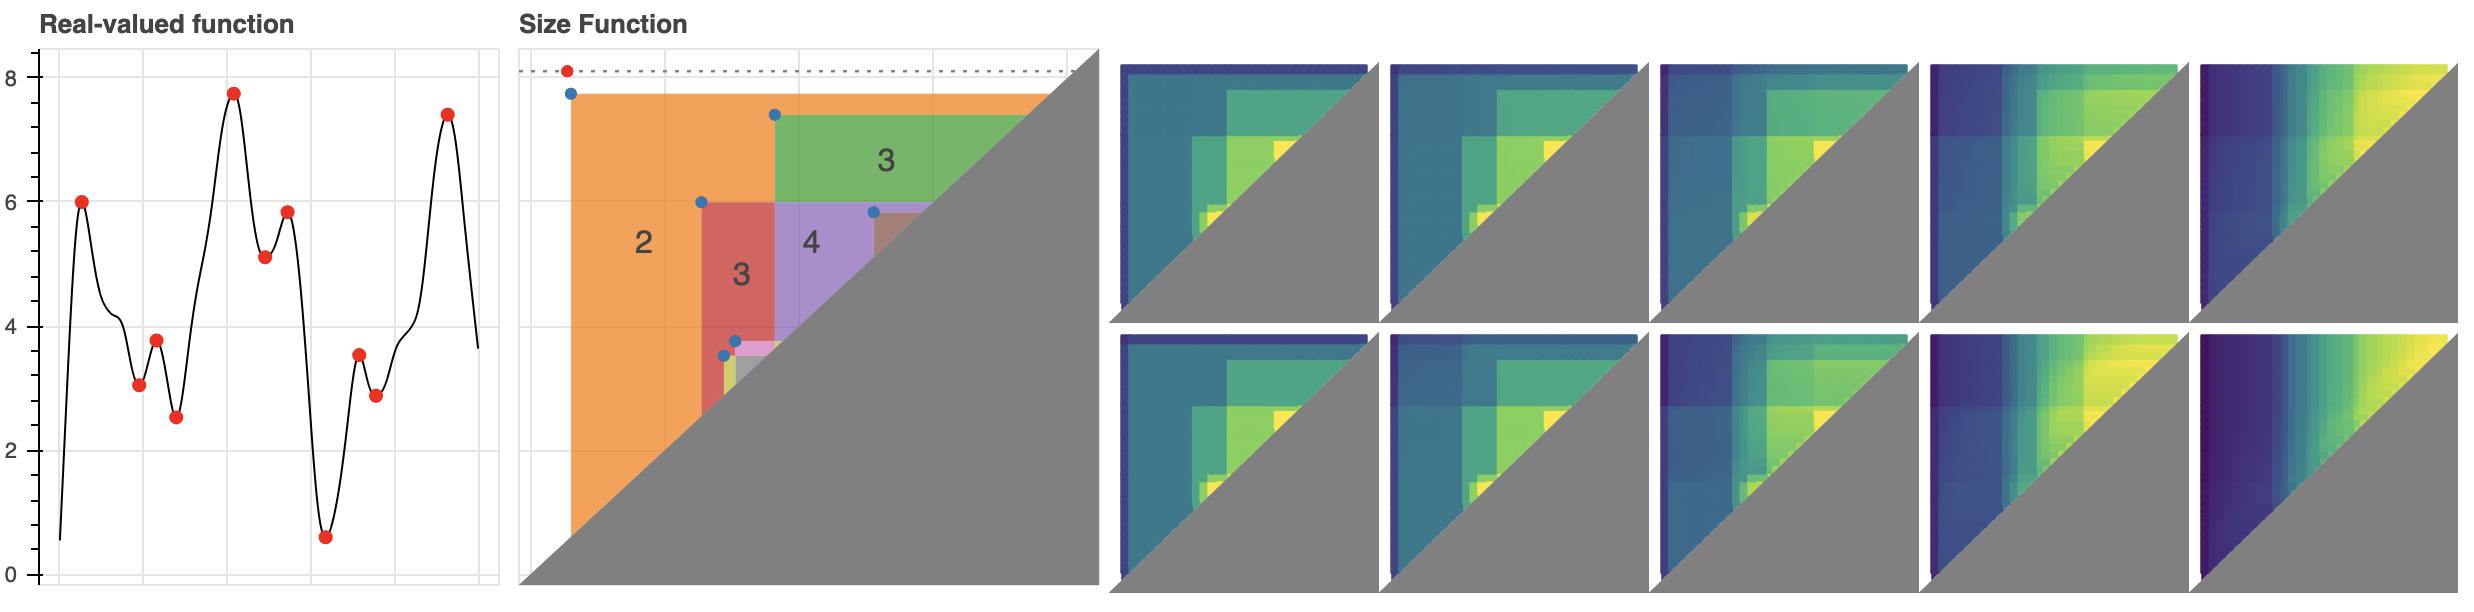
\includegraphics[width=0.95\textwidth]{../images/spectral_relax_size_func.png}	
\caption{ (left) A function $f: \mathbb{R} \to \mathbb{R}$ and its corresponding persistence diagram obtained by filtering $f$ by its sublevel sets. (right) Spectral interpolations to various Laplacian norms. }
\end{figure}

Though theoretically sound, diagrams suffer from many practical issues: they are sensitive to outliers, far from injective, and expensive---both to compute \textit{and} compare. Towards ameliorating these issues, practitioners have equipped diagrams with additional structure by way of maps to function spaces; examples include persistence images~\cite{adams2017persistence}, persistence landscapes~\cite{bubenik2015statistical}, and template functions~\cite{perea2022approximating}. Tackling the issue of injectivity, Turner et al.~\cite{turner2014persistent} propose an injective shape statistic of directional diagrams associated to a data set $X \subset \mathbb{R}^d$, sparking both an inverse theory for persistence and a mathematical foundation for metric learning. Despite the potential these extensions have in learning applications, scalability issues due to high algorithmic complexity remain. Indeed, this issue is compounded in the parameterized setting, where adaptations of the persistence computation has proven non-trivial~\cite{piekenbrock2021move}.

We seek to shift the computational paradigm on persistence while retaining its application potential: rather than following a construct-then-vectorize approach, we devise a spectral method that performs both steps, simultaneously and approximately. Our strategy is motivated both by a technical observation that suggests advantages exist for the rank invariant computation (\cite{sec:betti_derivation}) and by measure-theoretic results on $\mathbb{R}$-indexed persistence modules~\cite{cerri2013betti, chazal2016structure}, which generalize~\ref{eq:dgm} to rectangles $R = [a , b] \times [c , d] \subset \mathbb{R}^2$: 

%\begin{equation}\label{eq:measure}
%\mu_p^{R}(K, f) = \card \left( \restr{\dgm_p(K, f)}{R} \right) = \beta_p^{b,c} - \beta_p^{a,c} - \beta_p^{b,d} + \beta_p^{a,d}
%\end{equation}

Notably, our approach not only avoids explicitly constructing diagrams, but is also \textbf{matrix-free}, circumventing the reduction algorithm from~\cite{edelsbrunner2022computational} entirely. Additionally, the relaxation is computable exactly in linear space and quadratic time, requires no complicated data structures or maintenance procedures to implement, and can be iteratively $(1 \pm \epsilon)$ approximated in effectively linear time in practice for large enough $\epsilon > 0$. 

\textbf{Contributions:} Our primary contribution is the introduction of several families of spectral approximations to the rank invariants—$\mu_p$ and $\beta_p$—all of which are Lipshitz continuous, and differentiable on the positive semi-definite cone (\ref{prop:operator_props}). Leveraging the vast spectral theory that exists for Laplacian operators (\ref{sec:laplacian_theory2}), we show these approximations are computable in $O (m)$ memory and $O (m n)$ time, where $n$ ($m$) are the number of $p$ ($p + 1$, respectively) simplices in $K$ (\ref{prop:spectral_rank_complexity}). Moreover, both relaxations recover their corresponding invariants when $\epsilon$ is made small enough, and both admit iterative $(1 \pm \epsilon)$-approximation schemes (\ref{sec:iterative_approx}).  

\section{Notation \& Background}\label{sec:background_notation}

A \emph{simplicial complex} \(K \subseteq \mathcal{P}(V)\) over a finite set \(V = \{ v_{1},v_{2},\ldots,v_{n}\}\) is a collection of simplices \(\{\,\sigma:\sigma \in \mathcal{P}(V)\,\}\) such that \(\tau \subseteq \sigma \in K \Rightarrow \tau \in K\). A \emph{\(p\)-simplex} \(\sigma \subseteq V\) is a set of \(p + 1\) vertices, the collection of which is denoted as \(K^{p}\). An \emph{oriented \(p\)-simplex} \( [\sigma] \) is an ordered set \( [\sigma]  = ( - 1)^{|\pi|} \left[ v_{\pi(1)},v_{\pi(2)},\ldots,v_{\pi(p + 1)} \right] \), where \(\pi\) is a permutation on \( [\, p + 1\,]  = \{\, 1,2,\ldots,p + 1\,\}\) and \(|\pi|\) the number of its inversions. The \emph{\(p\)-boundary} \(\partial_{p} [\sigma] \) of an oriented \(p\)-simplex \( [\sigma]  \in K\) is defined as the alternating sum of its oriented co-dimension 1 faces, which collectively for all \(\sigma \in K^{p}\) define the \(p\)-th \emph{boundary matrix} \(\partial_{p}\) of \(K\):

\begin{equation*}
\partial_p[i, j] \triangleq 
\begin{cases}
(-1)^{s_{i j}} & \sigma_i \in \partial\left[\sigma_j\right] \\
0 & \text { otherwise }
\end{cases}, 
\quad \partial_p[\sigma] \triangleq \sum_{i=1}^{p+1}(-1)^{i-1} [v_1, \dots, v_{i-1}, v_{i+1}, \dots, v_{p+1}]
\end{equation*}\label{eq:alt_sum}
\noindent
where \(s_{ij} = \operatorname{sgn} \left(  \left[ \sigma_{i} \right] ,\partial \left[ \sigma_{j} \right]  \right) \) records the orientation. Extending \ref{eq:alt_sum} to all simplices in \(\sigma \in K\) for all \(p \leq \dim(K)\) yields the \emph{full boundary matrix} \(\partial\). With a small abuse in notation, we use \(\partial_{p}\) to denote both the boundary operator and its ordered matrix representative. When it is not clear from the context, we will clarify which representation is intended.

Generalizing beyond simplices, given a field \(\mathbb{F}\), an \emph{oriented \(p\)-chain} is a formal \(\mathbb{F}\)-linear combination of oriented \(p\)-simplices of \(K\) whose boundary \(\partial_{p} [ c] \) is defined linearly in terms of its constitutive simplices. The collection of \(p\)-chains under addition yields an \(\mathbb{F}\)-vector space \(C_{p}(K)\) whose boundaries \(c \in \partial_{p} [ c'] \) satisfying \(\partial_{p} [c]  = 0\) are called \emph{cycles}. Together, the collection of \(p\)-boundaries and \(p\)-cycles forms the groups \(B_{p}(K) = \mathrm{Im}\,\partial_{p + 1}\) and \(Z_{p}(K) = \mathrm{Ker}\,\partial_{p}\), respectively. The quotient space \(H_{p}(K) = Z_{p}(K)/B_{p}(K)\) is called the \emph{\(p\)-th homology group of \(K\)} with coefficients in \(\mathbb{F}\) and its dimension \(\beta_{p}\) is the \emph{\(p\)-th Betti number} of \(K\).

A \emph{filtration} is a pair \((K,f)\) where \(f:K \rightarrow I\) is a \emph{filter function} over an index set \(I\) satisfying \(f(\tau) \leq f(\sigma)\) whenever \(\tau \subseteq \sigma\), for any \(\tau,\sigma \in K\). For every pair \((a,b) \in I \times I\) satisfying \(a \leq b\), the sequence of inclusions \(K_{a} \subseteq \ldots \subseteq K_{b}\) induce linear transformations \(h_{p}^{a,b}:H_{p}\left( K_{a} \right) \rightarrow H_{p}\left( K_{b} \right)\) at the level of homology. When \(\mathbb{F}\) is a field, this sequence of homology groups uniquely decompose \((K,f)\) into a pairing \(\left( \sigma_{a},\sigma_{b} \right)\) demarcating the evolution of homology classes~\cite{zomorodian2004computing}: \(\sigma_{a}\) marks the creation of a homology class, \(\sigma_{b}\) marks its destruction, and the difference \(\left| {a - b} \right|\) records the lifetime of the class, called its \emph{persistence}. The persistent homology groups are the images of these maps and the persistent Betti numbers are their dimensions:

\[H_{p}^{a,b} = \begin{cases}
H_{p}\left( K_{a} \right) & \quad a = b \\
\operatorname{Im}\, h_{p}^{a,b} & \quad a < b
\end{cases}\:,\quad\quad\beta_{p}^{a,b} = \begin{cases}
\beta_{p}\left( K_{a} \right) & \quad a = b \\
\dim \left( H_{p}^{a,b} \right)  & \quad a < b
\end{cases}\]\protect\phantomsection\label{eq:pers_homology}{}

For a fixed \(p \geq 0\), the collection of persistent pairs \((a,b)\) together with unpaired simplices \((c,\infty)\) form a summary representation \(\operatorname{dgm}_{p}(K,f)\) called the \emph{\(p\)-th persistence diagram of \((K,f)\)}. Conceptually, \(\beta_{p}^{a,b}\) counts the number of persistent pairs lying inside the box \(( - \infty,a\,] \times (\, b,\infty)\)---the number of persistent homology groups born at or before \(a\) that died sometime after \(b\). When a given quantity depends on fixed parameters that are irrelevant or unknown, we use an asterisk. Thus, \(H_{p}^{\ast}(K)\) refers to any homology group of \(K\).

We will at times need to generalize the notation given thus far to the \emph{parameterized} setting. Towards this end, for some \(\mathcal{A} \subseteq \mathbb{R}^{d}\), we define an \emph{\(\mathcal{A}\)-parameterized filtration} as a pair \(\left( K,f_{\alpha} \right)\) where \(K\) is a simplicial complex and \(f:K \times \mathcal{A} \rightarrow \mathbb{R}\) an \(\mathcal{A}\)-parameterized filter function satisfying:
\begin{equation*}
f_{\alpha}(\tau) \leq f_{\alpha}(\sigma)\:\forall\:\tau \subseteq \sigma \in K\text{ and }f_{\alpha}(\sigma)\text{ is continuous in }\alpha \in \mathcal{A}\text{ for every }\sigma \in K
\end{equation*}
Intuitively, when \(\mathcal{A} = \mathbb{R}\), one can think of \(\alpha\) as a \emph{time} parameter and each \(f_{\alpha}(\sigma)\) as tracing a curve in \(\mathbb{R}^{2}\) parameterized by \(\alpha\). Examples of parameterized filtrations include:
\begin{itemize}
\item
  (Constant filtration) For a filter \(f:K \rightarrow \mathbb{R}\), note \(\left( K,f_{\alpha} \right)\) generalizes the ``static'' notion of a filtration \((K,f)\) in the sense one may declare \(f_{\alpha}(\sigma) = f(\sigma)\) for all \(\alpha \in \mathcal{A}\) and all \(\sigma \in K\).
\item
  (Dynamic Metric Spaces) For a set \(X\), let \(\gamma_{X} =  \left( X,d_{X} ( \cdot )  \right) \) denote a dynamic metric space~\cite{kim2021spatiotemporal}, where \(d_{X} ( \cdot ) :\mathbb{R} \times X \times X\) denotes a time-varying metric. For any fixed \(K \subset \mathcal{P}(X)\), the pair \(\left( K,f_{\alpha} \right)\) obtained by setting \(f_{\alpha}(\sigma) = \max\limits_{x,x' \in \sigma}d_{X}(\alpha)(x,x')\) recovers the notion of a \emph{time-varying Rips filtration}.
\item
  (Interpolating filtrations) For \(f,g:K \rightarrow \mathbb{R}\) filters over \(K\), a natural family of filtrations \(\left( K,h_{\alpha} \right)\) is obtained by choosing a homotopy \(h:\mathbb{R} \times [ 0,1] \rightarrow \mathbb{R}\) satisfying \(h_{0} = f\) and \(h_{1} = g\).
\end{itemize}

\begin{itemize}
\item
  (Fibered barcode) For a 2-d persistence module \(M\), a common invariant of interest is the \emph{fibered barcode}, which is the collection of barcodes of \(1\)-d affine slices of \(M\). These affine slices are themselves restrictions of a bifiltration parameterized by a 2-parameter family of lines homeomorphic to \([ 0,1] \times \mathbb{R}\)~\cite{lesnick2015interactive}.
\end{itemize}

\subsection{Technical background}\label{sec:betti_derivation}
The following results summarize some technical observations motivating this effort, which will be used in several proofs. Though these observations serve as background material, they contextualize our non-traditional computation of the rank invariant (\ref{cor::rank_reduction}) and serve as the motivation for this work.

Among the most widely known results for persistence is the structure theorem~\cite{zomorodian2004computing}, which shows 1-parameter persistence modules decompose in an \emph{essentially unique} way. Computationally, the corresponding Pairing Uniqueness Lemma~\cite{cohen2006vines} asserts that if \(R = \partial V\) decomposes the boundary matrix \(\partial \in \mathbb{F}^{N \times N}\) to a \emph{reduced} matrix \(R \in \mathbb{F}^{N \times N}\) using left-to-right column operations, then:
\begin{equation*}
	R [ i,j]  \neq 0 \Leftrightarrow \operatorname{rank} \left( \partial^{i,j} \right)  - \operatorname{rank} \left( \partial^{i\mathtt{+}1,j} \right)  + \operatorname{rank} \left( \partial^{i\mathtt{+}1,j\mathrm{-}1} \right)  - \operatorname{rank} \left( \partial^{i,j\mathrm{-}1} \right)  \neq 0
\end{equation*}\label{eq:uniq_pivot}
\noindent
where \(\partial^{i,j}\) denotes the lower-left submatrix defined by the first \(j\) columns and the last \(m - i + 1\) rows (rows \(i\) through \(m\), inclusive). Thus, the existence of non-zero ``pivot'' entries in \(R\) may be inferred entirely from the ranks of certain submatrices of \(\partial\). Part of the validity of \ref{eq:uniq_pivot} can be attributed to the following Lemma:

%#lemma[
%	Given filtration $(K , f)$ of size $N = abs(K)$, let $R = diff V$ denote the decomposition of the filtered boundary matrix $diff in bb(F)^(N times N)$. Then, for any pair $(i , j)$ satisfying $1 <= i lt j <= N$, we have: 
%
%	$ rank lr((R^(i , j))) = rank lr((diff^(i , j))) $ <eq:lower_left_rank>
%
%	Equivalently, all lower-left submatrices of $diff$ have the same rank as their corresponding submatrices in $R$.
%] <lemma:rank>


An explicit proof of both of these facts can be found in \cite{dey2022computational}, though the latter was also noted in passing by Edelsbrunner \cite{edelsbrunner2000topological}. Though typically viewed as minor facts needed to prove the correctness of the reduction algorithm, the implications of these two observations are are quite general, as recently noted by \cite{bauer2022keeping}:

%#corollary("Bauer et al. " + [@bauer2022keeping])[
%	Any persistence algorithm which preserves the ranks of the submatrices $diff^(i , j) (K , f)$ for all $i , j in lr([N])$ satisfying $1 <= i lt j <= N$ is a valid persistence algorithm.
%] <cor:valid_pers>

Indeed, though \(R\) is not unique, its non-zero pivots are, and these pivots \emph{define} the persistence diagram. Moreover, due to \ref{eq:lower_left_rank}, both \(\beta_{p}^{\ast}\) and \(\mu_{p}^{\ast}\) may be written as a sum of ranks of submatrices of \(\partial_{p}\) and \(\partial_{p + 1}\):

%#corollary[
%	Given a fixed $p >= 0$, a filtration $(K , f)$ with filtration values $brace.l thin a_i thin brace.r_(i = 1)^N$, and a rectangle $R = lr([a_i , a_j]) times lr([a_k , a_l]) subset Delta_+$, the persistent Betti and multiplicity functions may be written as:
%	$ beta_p^(a_i, a_j) (K, f) = rank(C_p (K_i)) - rank(partial_p^(1,i)) - rank(partial_(p+1)^(1,j)) - rank(partial_(p+1)^(i+1,j)) $ <eq:betti_four>
%	$ mu_p^R (K, f) = rank(partial_(p+1)^(j+1, k)) - rank(partial_(p+1)^(i+1, k)) - rank(partial_(p+1)^(j+1, l)) + rank(partial_(p+1)^(i+1, l)) $ <eq:mu_four>
%] <cor:rank_reduction>

Though \ref{eq:mu_four} was pointed out by Cohen-Steiner et al. in \cite{cohen2006vines} and exploited computationally by Chen \& Kerber in \cite{chen2011output}, to the authors knowledge the only explicit derivation and proof of \ref{eq:betti_four} is given by Dey \& Wang \cite{dey2022computational}. For completeness, we give our own detailed proof of \ref{cor:rank_reduction} in \ref{sec:proofs}. In practice, neither expressions seem used or even implemented in any commonly used persistence software.

Two important properties of the expressions from \ref{cor:rank_reduction} are: (1) they are comprised strictly of \emph{rank} computations, and (2) all terms involve \emph{unfactored} boundary matrices. Coupled with measure-theoretic perspectives on persistence \cite{chazal2016structure}, the former suggests variational perspectives of the rank function might yield interesting spectral relaxations of \ref{eq:betti_four} and \ref{eq:mu_four} useful for e.g. optimization purposes. Both the latter property with \ref{cor:valid_pers} suggests a potentially new means of computing persistence information \emph{without} matrix reduction. Moreover, combining these observations suggests advances made in other areas of applied mathematics may be readily exploited, such as the rich theory of matrix functions \cite{bhatia2013matrix}, the tools developed as part of ``The Laplacian Paradigm'' \cite{teng2010laplacian}, or the recent connections between rank and trace estimation \cite{ubaru2016fast}. The rest of the paper is dedicated to exploring these connections and their implications.

\subsection{Spectral relaxation and its implications}\label{sec:spectral_sec}

Before introducing our proposed relaxation, it is instructive to examine the how traditional expressions of the persistent rank invariants compare to those from \ref{cor:rank_reduction}. Given a filtration \((K,f)\) of size \(N = |K|\) with \(f:K \rightarrow I\) defined over some index set \(I\), its \(p\)-th persistent Betti number \(\beta_{p}^{a,b}\) at index \((a,b) \in I \times I\), is defined as follows:

\[\begin{aligned}
\beta_{p}^{a,b} & = \dim(Z_{p}\left( K_{a} \right)\:/\: B_{p}\left( K_{b} \right)) \\
 & = \dim(Z_{p}\left( K_{a} \right)\:/\:\left( Z_{p}\left( K_{a} \right) \cap B_{p}\left( K_{b} \right) \right)) \\
 & = \dim(Z_{p}\left( K_{a} \right)) - \dim(Z_{p}\left( K_{a} \right) \cap B_{p}\left( K_{b} \right))
\end{aligned}\] \protect\phantomsection\label{eq:pbn}{}

Computationally, observe that \ref{eq:pbn} reduces to one nullity computation and one subspace intersection computation. While the former is easy to re-cast as a spectral computation, computing the latter typically requires obtaining bases via matrix decomposition. Constructing these bases explicitly using conventional \cite{bhatia2013matrix} or persistence-based \cite{zomorodian2004computing}\cite{memoli2022persistent} algorithms effectively\footnote{An alternative means to perform matrix reduction is through the PLU factorization (see \cite{dey2022computational}, section 5.1.1), which takes \(O\left( n^{\omega} \right)\) time where \(\omega \in [ 2,2.373)\) is the matrix-multiplication constant. However, this approach exploits neither the structure of the boundary matrix nor properties of persistence to accelerate the computation and is not used in practice.} requires \(\Omega \left( N^{3} \right) \) time and \(\Omega \left( N^{2} \right) \) space. As the persistence algorithm also exhibits \(O \left( N^{3} \right) \) time complexity and completely characterizes \(\beta_{p}^{a,b}\) over \emph{all} values \((a,b) \in I \times I\), there is little incentive to compute \(\beta_{p}^{a,b}\) with such direct methods (and indeed, they are largely unused). Because of this, we will focus on expressions \ref{eq:betti_four} and \ref{eq:mu_four} throughout the rest of the paper.

\subsubsection{Parameterized boundary operators}\label{sec:param_boundary}

In typical dynamic persistence settings (e.g. \cite{cohen2006vines}), a decomposition \(R = \partial V\) of the boundary matrix \(\partial\) must be permuted and modified frequently to maintain a simplexwise order respecting \(f_{\alpha}\). In contrast, one benefit of the rank function is its permutation invariance: for any \(X \in \mathbb{R}^{n \times n}\) and permutation \(P\) we have: \[\operatorname{rank}(X) = \operatorname{rank} \left( P^{T}XP \right) \] This suggests persistent rank computations like those from \ref{cor:rank_reduction} need not maintain this ordering---as long as the constitutive boundary matrices the same non-zero pattern as their filtered counterparts, their ranks will be identical. In what follows, we demonstrate how exploiting this permutation invariance significantly simplifies the practical use of \ref{eq:betti_four} and \ref{eq:mu_four} in \emph{parameterized} settings.

Let \(\left( K,f_{\alpha} \right)\) denote parameterized family of filtrations of a simplicial complex of size \(\left| K^{p} \right| = n\). Fix an arbitrary linear extension \( (K, \preceq ) \) of the face poset of \(K\). Define the \(\mathcal{A}\)-\emph{parameterized} \emph{boundary operator} \({\hat{\partial}}_{p}(\alpha) \in \mathbb{R}^{n \times n}\) of \(\left( K,f_{\alpha} \right)\) as the \(n \times n\) matrix ordered by \(\preceq\) for all \(\alpha \in \mathcal{A}\) whose entries \((k,l)\) satisfy:

\[\partial_{p}(\alpha) [ k,l]  = \begin{cases}
s_{kl} \cdot f_{\alpha}\left( \sigma_{k} \right) \cdot f_{\alpha}\left( \sigma_{l} \right) & \quad\text{if }\sigma_{k} \in \partial_{p}\left( \sigma_{l} \right) \\
0 & \quad\text{otherwise}
\end{cases}\] \protect\phantomsection\label{eq:param_boundary_matrix}{}

where \(s_{kl} = \operatorname{sgn} \left(  \left[ \sigma_{k} \right] ,\partial \left[ \sigma_{l} \right]  \right) \) is the sign of the oriented face \( \left[ \sigma_{k} \right] \) in \(\partial \left[ \sigma_{l} \right] \). Observe that \ref{eq:param_boundary_matrix} may be decoupled into a product of diagonal matrices \(D_{\ast}\left( f_{\alpha} \right)\):

\[\partial_{p}(\alpha) \triangleq D_{p}\left( f_{\alpha} \right) \cdot \partial_{p} \left( K_{\preceq} \right)  \cdot D_{p + 1}\left( f_{\alpha} \right)\] \protect\phantomsection\label{eq:decouple}{}

where \(D_{p}\left( f_{\alpha} \right)\) and \(D_{p + 1}\left( f_{\alpha} \right)\) are diagonal matrices whose non-zero entries are ordered by restrictions of \(f_{\alpha}\) to \(K_{\preceq}^{p}\) and \(K_{\preceq}^{p + 1}\), respectively. Clearly, \(\operatorname{rank}\left( \partial_{p}(\alpha) \right) = \operatorname{rank} \left( \partial_{p} \left( K_{\preceq} \right)  \right) \) when the diagonal entries of \(D_{p}\) and \(D_{p + 1}\) are strictly positive. Moreover, observe we may restrict to those ``lower left'' matrices from \ref{lemma:rank} via post-composing step functions \[{\overline{S}}_{a}(x) = \mathbb{1}_{x > a}\] and \(S_{b}(x) = \mathbb{1}_{x \leq b}(x)\) to \(D_{p}\) and \(D_{p + 1}\), respectively:

\[{\hat{\partial}}_{p}^{a,b}(\alpha) \triangleq D_{p}\left( {\overline{S}}_{a} \circ f_{\alpha} \right) \cdot \partial_{p} \left( K_{\preceq} \right)  \cdot D_{p + 1}\left( S_{b} \circ f_{\alpha} \right)\] \protect\phantomsection\label{eq:rank_equiv_param}{}

Though these step functions are discontinuous at their chosen thresholds \(a\) and \(b\), we may retain the element-wise continuity of \ref{eq:decouple} by exchanging them with clamped \emph{smoothstep} functions \(\mathcal{S}:\mathbb{R} \rightarrow  [ 0,1] \) that interpolate the discontinuous step portion of \(S\) along a fixed interval \((a,a + \omega)\), for some \(\omega > 0\) (see \ref{fig:smoothstep}).

The observations above collectively motivate our first relaxation. Without loss in generality, assume the orientation of the simplices \( (K, \preceq ) \) is induced by the order on the vertex set \(V\). To simplify the notation, we write \(A^{x} = A^{\ast ,x}\) to denote the submatrix including all rows of \(A\) and all columns of \(A\) up to \(x\).

Note that in \ref{eq:rank_equiv_param}, we write \(\partial_{p} \left( K_{\preceq} \right) \) (as opposed to \(\partial_{p}(K,f)\)) to emphasize \(\partial_{p} \left( K_{\preceq} \right) \) is ordered according to a fixed linear ordering \( (K, \preceq ) \). The distinction is necessary as evaluating the boundary terms from \ref{cor:rank_reduction} would require \(\partial\) to be explicitly filtered in the total ordering induced by \(f_{\alpha}\)---which varies in \(\mathcal{A}\)---whereas the expressions obtained by replacing the constitutive terms in \ref{eq:betti_four} and \ref{eq:mu_four} with \ref{eq:pbn_parameterized} and \ref{eq:mu_parameterized}, respectively, requires no such explicit filtering.

\subsection{Parameterized Laplacians}\label{sec:laplacian_theory2}

For generality's sake, it is important to make the class of expressions for \(\beta_{p}^{\ast}\) and \(\mu_{p}^{\ast}\) as large as possible. Since we are only concerned with homology over \(\mathbb{R}\), we may exploit another identity of the rank function which is only applicable to zero characteristic fields:

\[\operatorname{rank}(X) = \operatorname{rank} \left( XX^{T} \right)  = \operatorname{rank} \left( X^{T}X \right) ,\quad\text{for all }X \in \mathbb{F}^{n \times m}\] \protect\phantomsection\label{eq:rank_invariance_adjoint}{}

In the context of boundary operators, note that \(\partial_{1}\partial_{1}^{T}\) is the well known \emph{graph Laplacian}---more generally, \ref{eq:rank_invariance_adjoint} suggests we can readily express \(\beta_{p}^{\ast}(\alpha)\) and \(\mu_{p}^{\ast}(\alpha)\) using the ranks of combinatorial \(p\)-Laplacians.\footnote{By convention, we define \(\partial_{p} = 0\) for all \(p \leq 0\).}

Following the seminal results from Horak and Jost \cite{horak2013spectra}, there are three natural ways to define \(p\)-Laplacians over a fixed simplicial complex \(K\): the \emph{up}-Laplacian \(L_{p}^{\operatorname{up}}(K)\), the \emph{down}-Laplacian \(L_{p}^{\operatorname{dn}}(K)\), and their sum, which we refer to as the \emph{combinatorial} Laplacian \(\Delta_{p}(K)\):

\[\Delta_{p}(K) = \underset{L_{p}^{\operatorname{up}}}{\underbrace{\partial_{p + 1} \circ \partial_{p + 1}^{T}}} + \underset{L_{p}^{\operatorname{dn}}}{\underbrace{\partial_{p}^{T} \circ \partial_{p}}}\] \protect\phantomsection\label{eq:comb_lap}{}

All three operators \(\Delta_{p}\), \(L_{p}^{\operatorname{up}}\), and \(L_{p}^{\operatorname{dn}}\) are symmetric, positive semi-definite, and compact \cite{memoli2022persistent}---moreover, the \emph{non-zero} multisets \(\Lambda \left( L_{p}^{\operatorname{up}} \right) \) and \(\Lambda \left( L_{p + 1}^{\operatorname{dn}} \right) \) are equivalent, implying they must have identical ranks (see Theorem 2.2 and 3.1 of \cite{horak2013spectra}). Thus, for rank computations, it suffices to consider only one of them.

Let \(\left( K,f_{\alpha} \right)\) denote a parameterized family of filtrations of a simplicial complex \(K\) equipped with a fixed but arbitrary linear extension \(\preceq\) of its face poset and fixed orientations \(s(\sigma)\) inherited from the total order on the vertex set \( (V, \preceq ) \). Without loss of generality, we define the weighted \(p\) up-Laplacian \(\mathcal{L}_{p} \triangleq L_{p}^{\operatorname{up}}\) at index \((a,b)\) as follows:

\[\begin{aligned}
\mathcal{L}_{p, \preceq}^{a,b}(\alpha) & \triangleq D_{p}\left( {\overline{S}}_{a} \circ f_{\alpha} \right) \cdot \partial_{p + 1} \left( K_{\preceq} \right)  \cdot D_{p + 1}\left( S_{b} \circ f_{\alpha} \right) \cdot \partial_{p + 1}^{T} \left( K_{\preceq} \right)  \cdot D_{p}\left( {\overline{S}}_{a} \circ f_{\alpha} \right)
\end{aligned}\] \protect\phantomsection\label{eq:laplacian_decouple}{}

where \(D_{p}(f)\) denotes a diagonal matrix whose entries represent the application of \(f\) to the \(p\)-simplices of \(K\). As in \ref{eq:rank_equiv_param}, fixing step function \(S_{a}\) and \({\overline{S}}_{b}\) at values \(a,b \in \mathbb{R}\) yields operators whose ranks correspond to the ranks of certain ``lower-left'' submatrices of the corresponding full boundary matrix \(\partial\) of \((K,f)\). In particular, if \(R = \partial V\) is the decomposition of \(\left( K,f_{\alpha} \right)\) for some fixed choice of \(\alpha \in \mathcal{A}\), then for any pair \((a,b) \in \Delta_{+}\) there exists indices \(i = \sum_{\sigma \in K}\left( {\overline{S}}_{a} \circ f_{\alpha} \right)(\sigma)\) and \(j = \sum_{\sigma \in K}\left( S_{b} \circ f_{\alpha} \right)(\sigma)\) such that:

\[\operatorname{rank} \left( R_{p + 1}^{i,j} \right)  = \operatorname{rank} \left( \partial_{p + 1}^{i,j} \right)  = \operatorname{rank} \left( {\hat{\partial}}_{p + 1}^{a,b} \right)  = \operatorname{rank} \left(  \left( {\hat{\partial}}_{p + 1}^{a,b} \right)  \left( {\hat{\partial}}_{p + 1}^{a,b} \right) ^{T} \right)  = \operatorname{rank} \left( \mathcal{L}_{p, \preceq}^{a,b} \right) \]

where the second last equality uses the identity \(\operatorname{rank}(X) = \operatorname{rank} \left( X^{T}X \right) \), which is true when \(X \in \mathbb{F}^{n \times m}\) has coefficients in a zero-characteristic field \(\mathbb{F}\). This confirms that we may substitute any of the parameterized boundary operators used in \ref{prop:mu_betti_1} with weighted Laplacian operators \(\partial_{p + 1}^{\ast} \mapsto \mathcal{L}_{p}^{\ast}\) equipped with the appropriate down- and up-step functions \(S_{\ast}\) and \({\overline{S}}_{\ast}\), respectively.

It is worth noting that composing step functions \({\overline{S}}_{a},S_{b}:\mathbb{R} \rightarrow  [ 0,1] \) with \(f_{\alpha}\) is equivalent to endowing a \emph{weight function} \(w:K \rightarrow (0, + \infty)\) on a subset \(K_{a,b} \subseteq K\), in the sense described by \cite{memoli2022persistent}. In particular, if \(w_{p}\) denotes the restriction of \(w\) to \(K^{p}\), then \(w_{p}\) defines an inner product \(\langle\, \cdot , \cdot \,\rangle_{w_{p}}\) on space of \(p\)-chains \(C_{p}\left( K,\mathbb{R} \right)\) given by:

\[\langle [\sigma] , [\sigma'] \rangle_{w_{p}} \triangleq \delta_{\sigma\sigma'} \cdot \left( w_{p}(\sigma) \right)^{- 1},\quad\forall\,\sigma,\sigma' \in K^{p}\] \protect\phantomsection\label{eq:inner_product_chain}{}

where \(\delta_{\sigma\sigma'} = \mathcal{1} (\sigma = \sigma') \) is the indicator function on \(\sigma\). Moreover, this inner product \(\langle [\sigma] , [\sigma'] \rangle_{w_{p}}\) on \(C_{p}\left( K,\mathbb{R} \right)\) induces an inner product:

%\[《f,g》_{w} = \sum_{\sigma \in K^{p}}f\left( [\sigma] \right)g\left( [\sigma] \right)w(\sigma),\quad\text{for all }f,g \in C^{p}(K)\]\protect\phantomsection\label{eq:inner_product_cochain}{}

In these sense above, \ref{eq:laplacian_decouple} is simply choosing a particular inner product on the space of \(p\)-cochains.

% === 
\section{Spectral rank relaxation}\label{sec:spectral_relax}

Under mild assumptions on \(f_{\alpha}\), the entries of the boundary operators from \ref{eq:rank_equiv_param} are continuous functions of \(\alpha\) when \(S\) is substituted appropriately with smooth step functions. In contrast, the quantities from \ref{prop:mu_betti_1} are by definition discontinuous functions, as they are integer-valued due to the rank function. To circumvent this issue, we consider the spectral characterization of the rank function:

\[\operatorname{rank}(X) = \sum_{i = 1}^{n}\operatorname{sgn}_{+}\left( \sigma_{i}(X) \right),\quad\quad\operatorname{sgn}_{+}(x) = \begin{cases}
\: 1 & \quad\text{if }x > 0 \\
\: 0 & \quad\text{otherwise}
\end{cases}\] \protect\phantomsection\label{eq:rank_def}{}

In the above, \(\{\sigma_{i}\}_{i = 1}^{n}\) are the singular values \(\Sigma = \operatorname{diag} \left( \{\sigma_{i}\}_{i = 1}^{n} \right) \) from the singular value decomposition (SVD) \(X = U\Sigma V^{T}\) of \(X \in \mathbb{R}^{n \times m}\), and \(\operatorname{sgn}_{+}:\mathbb{R} \rightarrow \{ 0,1\}\) is the one-sided sign function. As the singular values vary continuously under perturbations in \(X\) \cite{bhatia2013matrix}, it is clear the discontinuity in \ref{eq:rank_def} manifests from the one-sided sign function---thus, a natural approach to relaxing \ref{eq:rank_def} is to first relax the \(\operatorname{sgn}_{+}\) function.

Our approach follows the seminal work of Mangasarian et al. \cite{mangasarian1994class}. Let \(p:\mathbb{R}_{+} \rightarrow \mathbb{R}_{+}\) denote a continuous density function and \(\nu:\mathbb{R}_{+} \rightarrow \mathbb{R}_{+}\) is a continuous increasing function satisfying \(\nu(0) = 0\). One way to approximate the \(\operatorname{sgn}_{+}\) function is to integrate \(\tau\)-smoothed variations \(\hat{\delta}\) of the Dirac delta measure \(\delta\):

\[\phi(x,\tau) = \int_{- \infty}^{x}\hat{\delta}(z,\tau)\operatorname{dz},\quad\hat{\delta}(z,\tau) = \frac{1}{\nu(\tau)} \cdot p\left( \frac{z}{\nu(\tau)} \right),\quad\forall z \geq 0,\tau > 0\] \protect\phantomsection\label{eq:phi}{}

In contrast to the \(\operatorname{sgn}_{+}\) function, if \(p\) is continuous on \(\mathbb{R}_{+}\) then \(\phi ( \cdot ,\tau) \) is continuously differentiable on \(\mathbb{R}_{+}\), and if \(p\) is bounded above on \(\mathbb{R}_{+}\), then \(\phi ( \cdot ,\tau) \) is globally Lipshitz continuous on \(\mathbb{R}_{+}\). Moreover, varying \(\tau \in \mathbb{R}_{+}\) in \ref{eq:phi} yields an \(\tau\)-parameterized family of continuous \(\operatorname{sgn}_{+}\) relaxations \(\phi:\mathbb{R}_{+} \times \mathbb{R}_{+ +} \rightarrow \mathbb{R}_{+}\), where \(\tau > 0\) controls the accuracy of the relaxation.

Many properties of the sign approximation from \ref{eq:phi} extend naturally to the rank function when substituted appropriately via \ref{eq:rank_def}. In particular, pairing \(X = U\Sigma V^{T}\) with a scalar-valued \(\phi\) that is continuously differentiable at every entry \(\sigma\) of \(\Sigma\) yields a corresponding \emph{Löwner operator} \(\Phi_{\tau}\) \cite{bi2013approximation}:

\[\Phi_{\tau}(X) \triangleq \sum_{i = 1}^{n}\phi\left( \sigma_{i},\tau \right)u_{i}v_{i}^{T}\] \protect\phantomsection\label{eq:lowner}{}

Note that when \(X\) is positive semi-definite, \ref{eq:lowner} may be interpreted as a particular choice of \emph{matrix function} \(f(X) \triangleq Uf(\Lambda)U^{T}\) from the matrix function calculus perspective \cite{bhatia2013matrix}. Unlike general matrix functions, however, the restrictions on \(\phi\) \ref{eq:phi} grants the operators \(\Phi_{\tau}\) a variety of attractive properties related to approximation, monotonicity, and differentiability.

Noting property (4), since the sum Lipshitz functions is also Lipshitz, it is easy to verify that replacing the rank function in all of the constitutive terms from \ref{prop:mu_betti_1} yields Lipshitz continuous functions whenever the filter function \(f_{\alpha}\) is itself Lipshitz and the step functions from \ref{eq:rank_equiv_param} are smoothed (\(\omega > 0\)).

\textbf{Interpretation \#1:} In many applications, it is common to regularize an ill-posed objective function to encourage simpler solutions or to prevent overfitting. For example, the classical least-squares approach to solving the linear system \(Ax = b\) is often augmented with the \emph{Tikhonov regularization} (TR) for some \(\tau > 0\):

\[x_{\tau}^{\ast} = \text{ arg min}_{x \in \mathbb{R}^{n}}\left\| {Ax - b} \right\|^{2} + \tau\left\| x \right\|^{2} =  \left( A^{T}A + \tau I \right) ^{- 1}A^{T}b\] \protect\phantomsection\label{eq:tikhonov}{}

When \(\tau = 0\), one recovers the standard \(\ell_{2}\) minimization, whereas when \(\tau > 0\) solutions \(x_{\tau}^{\ast}\) with small norm are favored. Similarly, by parameterizing \(\phi\) by \(\nu(\tau) = \sqrt{\tau}\) and \(p(x) = 2x \left( x^{2} + 1 \right) ^{- 2}\), one obtains via \ref{eq:phi}:

\[\phi(x,\tau) = \int_{0}^{z}\hat{\delta}(z,\tau)dz = \frac{2}{\tau}\int_{0}^{z}z \cdot \left( \left( z/\sqrt{\tau} \right)^{2} + 1 \right)^{- 2}dz = \frac{x^{2}}{x^{2} + \tau}\] \protect\phantomsection\label{eq:tikhonov_sf}{}

By substituting \(\operatorname{sgn}_{+} \mapsto \phi\) and composing with the singular value function \ref{eq:lowner}, the corresponding spectral rank approximation reduces\footnote{See Theorem 2 of \cite{zhao2012approximation} for a proof of the second equality.} to the following \emph{trace} formulation:

\[\left\| {\Phi_{\tau}(A)} \right\|_{\ast} = \sum_{i = 1}^{n}\frac{\sigma_{i}(A)^{2}}{\sigma_{i}(A)^{2} + \tau} = \operatorname{tr} \left[  \left( A^{T}A + \tau\, I \right) ^{- 1}A^{T}A \right] \] \protect\phantomsection\label{eq:tikhonov_1}{}

The relaxation level \(\tau\) may be thought of as a regularization term that preferences smaller singular values: larger values smooth out \(\left\| {\Phi_{\tau} ( \cdot ) } \right\|_{\ast}\) by making the pseudo-inverse less sensitive to perturbations, whereas smaller values lead to a more faithful\footnote{This can be seen directly by \ref{eq:tikhonov} as well, wherein increasing \(\tau\) lowers the condition number of \(A^{T}A + \tau I\) monotonically, signaling a tradeoff in stability at the expense of accuracy.} approximations of the rank. In this sense, we interpret the quantities obtained by applying \ref{eq:lowner} to the terms from \ref{prop:mu_betti_1} as \emph{regularized RI approximation}.

\textbf{Interpretation \#2:} In spectral graph theory, matrix functions are often used to simulate diffusion processes on meshes or graphs embedded in \(\mathbb{R}^{d}\) to obtain information of about their geometry. For example, consider a weighted graph \(G = (V,E)\) with \(n = |V|\) vertices with graph Laplacian \(L_{G} = \partial_{1}\partial_{1}^{T}\). The \emph{heat} of every vertex \(v(t) \in \mathbb{R}^{n}\) as a function of time \(t \geq 0\) is governed by \(L_{G}\) and the \emph{heat equation}:

\[v'(t) = - L_{G}v(0)\quad \Leftrightarrow \quad L_{G} \cdot u(x,t) = - \partial u(x,t)/\partial t\] \protect\phantomsection\label{eq:heat_eq}{}

To simulate a diffusion process on \(G\) from an initial distribution of heat \(v(0) \in \mathbb{R}^{n}\), it suffices to construct the \emph{heat kernel} \(H_{t} \triangleq \exp \left( - t \cdot L_{G} \right) \) via the spectral decomposition \(L_{G} = U\Lambda U^{T}\) of \(L_{G}\):

\[v(t) = H_{t}\, v(0),\text{ where }H_{t} = \sum_{i = 1}^{n}e^{- t\lambda_{i}}\, u_{i}\, u_{i}^{T}\] \protect\phantomsection\label{eq:heat_kernel}{}

The heat kernel is invariant under isometric deformations, stable under perturbations, and is known to contain multiscale geometric information due to its close connection to geodesics. As is clear from \ref{eq:heat_kernel}, it is also a matrix function. Now, consider \ref{eq:phi} with \(\nu(\tau) = \tau\) and \(p(\lambda) = \exp\left( - \lambda_{+} \right)\) where \(x_{+} = \max(x,0)\):

\[\phi(\lambda,\tau) = \int_{0}^{z}\hat{\delta}(z,\tau)dz = \frac{1}{\tau}\int_{0}^{z}\exp( - z/\tau)dz = 1 - \exp( - \lambda/\tau),\quad\text{ for all }\lambda \geq 0\] \protect\phantomsection\label{eq:heat_sf}{}

In the context of diffusion, observe the parameter \(\tau\) is inversely related diffusion time (i.e. \(t = 1/\tau\)) and that as \(t \rightarrow 0\) (or \(\tau \rightarrow \infty\)) the expression \(1 - \exp( - \lambda/\tau)\) approaches the \(\operatorname{sgn}_{+}\) function on the interval \([ 0,\infty)\). As above, substituting \(\phi\) appropriately into \ref{eq:lowner} again yields an equivalent trace expression:

\[\left\| {\Phi_{\tau}\left( L_{G} \right)} \right\|_{\ast} = \sum_{i = 1}^{n}1 - \exp\left( - \lambda_{i}/\tau \right) = n - \operatorname{tr} \left[ H_{1/\tau} \right] \] \protect\phantomsection\label{eq:heat_trace}{}

The heat kernel \(H_{t}\) has been shown to fully characterize shapes up to isometry, motivating the creation of various geometric signatures, such as the Heat Kernel Signature (HKS) and the Heat Kernel Trace. In this sense, we interpret a spectral rank relaxation using \ref{eq:heat_sf} as a \emph{geometrically informative RI approximation}.


\section{Introduction}\label{sec1}

\backmatter

\bmhead{Supplementary information}
\bmhead{Acknowledgements}
\section*{Declarations}

%Some journals require declarations to be submitted in a standardised format. Please check the Instructions for Authors of the journal to which you are submitting to see if you need to complete this section. If yes, your manuscript must contain the following sections under the heading `Declarations':
%
%\begin{itemize}
%\item Funding
%\item Conflict of interest/Competing interests (check journal-specific guidelines for which heading to use)
%\item Ethics approval and consent to participate
%\item Consent for publication
%\item Data availability 
%\item Materials availability
%\item Code availability 
%\item Author contribution
%\end{itemize}

\noindent
If any of the sections are not relevant to your manuscript, please include the heading and write `Not applicable' for that section. 

\begin{appendices}

\section{Section title of first appendix}\label{secA1}

An appendix contains supplementary information that is not an essential part of the text itself but which may be helpful in providing a more comprehensive understanding of the research problem or it is information that is too cumbersome to be included in the body of the paper.

\end{appendices}

\bibliography{references}

\end{document}
